% Set the stage on AI systems
\label{sec:introduction:preface}

Within the last half-decade, we have seen an explosion of cloud-based services typically marketed under an \gls{ai} banner. 
Vendors are rapidly pushing out \gls{ai}-based solutions, technologies and products that encapsulate half a century worth of machine-learning research: a \citeyear{LoGiudice:2016wf} report by market research company Forrester captured such growth into four key areas \citep{LoGiudice:2016wf} as replicated in  \cref{fig:introduction:ai-products}. 
Application developers are eager to develop the next generation of `\gls{ai}-first' software, that will reason, sense, think, act, listen, speak and execute every whim in our web browser or smartphone app.
%A wave of \gls{ai}-first thinking embedded in companies' product lines is spearheaded through work achieved at Google, Microsoft and Facebook; for instance, Google's 2018 rebranding of \textit{Google Research} to \textit{Google AI} \citep{Howard:2018tz} or how \gls{ai} is leveraged \textit{at scale} within Facebook's infrastructure and platforms to serve its users with an \gls{ai}-first attitude \citep{Parekh:2017hx}.
%These services aim to lower the entry barrier to develop, test and deploy \gls{ai}-first software in both skill and time. 
%Application developers needn't require a formal training in \gls{ml} nor a strong understanding of mathematics: thus, \textit{skill required} is reduced. The training of such classifiers involves the laborious process of sourcing, curating and labelling large datasets: using such services does not, and thus \textit{time} is reduced. The process is abstracted behind an \glsac{api} call, only requiring knowledge on how to use a \glsac{rest}ful architecture \citep{Fielding:2000vh} (or similar) to access the cloud-based service.

An important contrast is how these systems begin to shift away from the traditional software engineering paradigm application developers are used to. As we unpack in \cref{sec:introduction:motivation,sec:background:probabilistic-stochastic}, typical systems built by application developers are \textit{rule-driven} (or algorithm-driven), deterministically human engineered using source code to drive each step behind the application. These rule-driven systems typically consume, utilise, and integrate libraries and frameworks, \glsacpl{ide} and other tooling, and cloud-based services such as \gls{aws} \citep{AWS:Home}. The \gls{ai}-first software is, however, not rule-driven but \textit{data-driven}, fuelled with large datasets used to train \gls{ml} prediction algorithms and classifiers that present a typically probabilistic and nondeterministic behaviour.

So, how does the application developer approach her \gls{ai}-first application? 

\begin{enumerate}
  \item She writes her own \gls{ml} classifier from scratch and trains it from her own curated dataset. This approach is laborious in time and demands formal training in \gls{ml} and mathematical knowledge, but the tradeoff is that she has full autonomy over the models she creates.
  \item She downloads a pre-trained model and `plugs' it into an existing \gls{ml} framework, such as Tensorflow \citep{Tensorflow:Whitepaper}. While this approach is less demanding in time, it still requires an understanding of how to `glue' the \gls{ml} framework code\footnote{Thus introducing a verbose list of \gls{ml} terminology to her already-required developer vocabulary. See a list of 328 terms provided by Google here: \url{https://developers.google.com/machine-learning/glossary/}.} with her own application code.
  \item She uploads her data to a pre-existing cloud-based service. She doesn't need to know anything behind the underlying `intelligence' and how it works, is fast to integrate into her application and all abstracted behind a web-based \gls{api} call.
\end{enumerate}

\noindent
At first sight, she perceives the data-driven cloud service as `just another' cloud service  offered in her toolchain. Her perception is that just because this is another cloud service, it should act and behave as any other typical service would. But internally, she isn't aware that it this particular cloud service isn't a typical one; the data-driven service does not adapt to her rule-driven application in the way that she thinks (\cref{fig:introduction:rule-vs-data}). This is because the nature of typical cloud systems and data-driven ones are not exactly the same (\cref{tab:introduction:characteristics-of-cloud}).

\begin{figure}[h!]
\centering
\caption[Data-driven cloud services are not the same as rule-driven ones]{The application developer's rule-driven toolchain is distinct from data-driven toolchain. A developer must consume a typical, data-driven cloud service in a different way than an intelligent data-driven cloud service as they are not the same type of system.}
\label{fig:introduction:rule-vs-data}
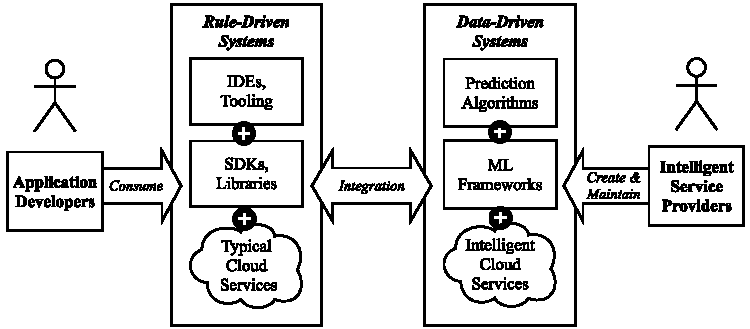
\includegraphics{rule-vs-data}
\end{figure}

\begin{table}[p]
\centering
\caption[Differing characteristics of cloud services]{Differing characteristics of intelligent and typical cloud services.}
\label{tab:introduction:characteristics-of-cloud}
\begin{tabular}{@{}ll@{}}
\toprule
  % Heading
  \textbf{Intelligent Cloud Services} &
  \textbf{Typical Cloud Services}
  \\
  \midrule
  Probabilistic &
  Deterministic 
  \\
  Machine Learnt &
  Human Engineered
  \\
  Data-Driven &
  Rule-Driven
  \\
  Black-Box &
  Mostly Transparent
  \\
  \bottomrule
\end{tabular}
\end{table}


This `range' of \gls{ai}-first integration techniques partially reflects Google AI's\footnote{
Google AI was recently rebranded from Google Research, further highlighting how the `\gls{ai}-first' philosophy is increasingly becoming embedded in companies' product lines and research and development teams. Spearheaded through work achieved at Google, Microsoft and Facebook, the emphasis can be seen through Google's 2018 rebranding of \textit{Google Research} to \textit{Google AI} \citep{Howard:2018tz} or how \gls{ai} is leveraged \textit{at scale} within Facebook's infrastructure and platforms to serve its users with an \gls{ai}-first attitude \citep{Parekh:2017hx}.
} 
\textit{\acrlong{ml} Spectrum} \citep{Ortiz:2017wg,LaForge:2018tm,McGowen:2019vt}, which encompasses the variety of skill, effort, users and types of outputs of integration techniques. On one extreme is the research of developing algorithms to achieve intelligence, produced chiefly in academia---coined as \gls{byoml} \citep{Ortiz:2017wg,McGowen:2019vt,Jimerson:2017vh}. On the other, such intelligence becomes heavily abstracted as easy-to-use \glspl{api}, targeted mainly towards developers as `friendly' \gls{ml}. In the middle lies a broad mix of combining both cloud and locally-hosted solutions (with varying levels of automation to assist in development) that turn custom datasets into some form of predictive intelligence. 

All techniques in this spectrum are data-driven, and we illustrate their slightly varied characteristics further in \cref{tab:introduction:comparison-of-ml-spectrum} and examples of the computer vision spectrum in \cref{fig:introduction:cv-spectrum}.

\begin{figure}[h!]
\centering
\caption[Examples of the machine learning spectrum in computer vision]{Examples within the machine learning spectrum of computer vision. Benefits and drawbacks of each end of the spectrum are indicated with the colour scales.}
\label{fig:introduction:cv-spectrum}
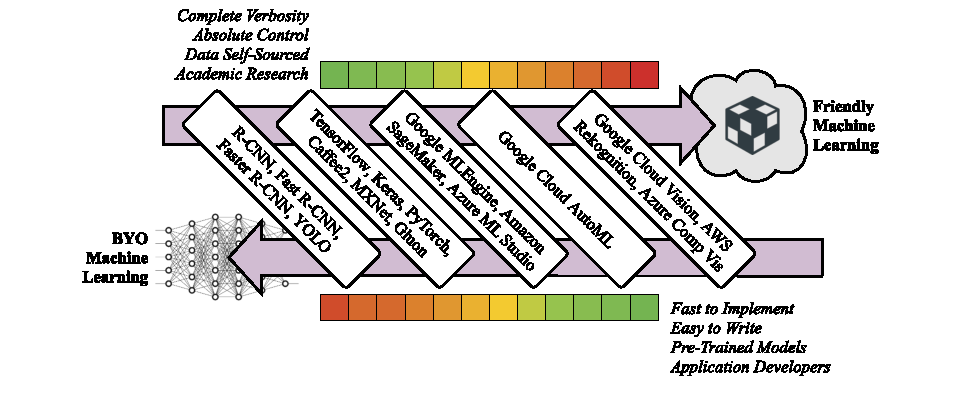
\includegraphics[width=\linewidth]{cv-spectrum}
\end{figure}

\begin{table}[p]
\centering
\caption[Comparison of the machine learning spectrum]{Comparison of the machine learning spectrum.}
\label{tab:introduction:comparison-of-ml-spectrum}
\begin{tabular}{@{}l|ccccc@{}}
\toprule
  % Heading
  \textbf{Comparator} &
  \textbf{\glsac{byoml}} &
  \textbf{\glsac{ml} F'work} &
  \textbf{Cloud \glsac{ml}} &
  \textbf{Auto-Cloud \glsac{ml}} &
  \textbf{Cloud \glsac{api}} 
  \\ 
  \midrule
  \thinrule
  % Hosting
  \textbf{Hosting} & & & & & \\
  \thinrule
    Locally & \checkmark & \checkmark &  &  &  \\
    Cloud &  &  & \checkmark & \checkmark & \checkmark \\
  \midrule
  \thinrule
  % Output Type
  \textbf{Output} &  &  &  &  &  \\
  \thinrule
    Custom Model & \checkmark & \checkmark & \checkmark & \checkmark &  \\
    \glsac{http} Response &  &  &  &  & \checkmark \\
  \midrule
  \thinrule
  % Autonomy
  \textbf{Autonomy} &  &  &  &  &  \\
  \thinrule
    Low &  &  &  &  & \checkmark \\
    Medium &  &  &  & \checkmark &  \\
    High &  & \checkmark & \checkmark &  &  \\ 
    Highest & \checkmark &  &  &  &  \\
  \midrule
  \thinrule
  % TTM
  \textbf{Time To Market} &  &  &  &  &  \\
  \thinrule
    Medium & \checkmark & \checkmark &  &  &  \\
    High &  &  & \checkmark & \checkmark &  \\
    Highest &  &  &  &  & \checkmark \\
  \midrule
  \thinrule
  % Data Source
  \textbf{Data} &  &  &  &  &  \\ 
  \thinrule
    Self-Sourced & \checkmark & \checkmark & \checkmark & \checkmark &  \\
    Pre-Trained &  & \checkmark &  &  & \checkmark \\
  \midrule
  \thinrule
  % Intended User
  \textbf{Intended User} &  &  &  &  &  \\
  \thinrule  
    Academics & \checkmark & \checkmark &  &  &  \\
    Data Scientist & \checkmark & \checkmark & \checkmark & \checkmark &  \\
    Developers &  &  &  & \checkmark & \checkmark \\
  \bottomrule
\end{tabular}
\end{table}

\itshape
In this study, we advocate that the (i)~integration, (ii)~documentation, and (iii)~quality attributes of data-driven cloud services juxtaposes the rule-driven nature of end-applications as these intelligent cloud services are vastly different to their traditional counterparts, and great care must therefore be considered by application developers.
\upshape
\bigskip

These cloud services have begun to gain traction within developer circles: \cref{fig:introduction:stackoverflow-trends} shows the increasing trend of posts since 2014 on Stack Overflow that categorise popular computer vision cloud \glspl{api}.\footnote{Query run on 12 October 2018 using StackExchange Data Explorer. Refer to \url{https://data.stackexchange.com/stackoverflow/query/910188} for full query.} In academia, these `off-the-shelf' and pre-packaged \gls{ml} solutions present a varied nomenclature such as \textit{Cognitive Applications} and \textit{Machine Learning Services} \citep{Hwang:2017tr} or \textit{Machine Learning as a Service} \citep{Ribeiro:2015dz}. Some services provide the infrastructure to rapidly begin training from custom datasets (Google's AutoML\footnoteurl{https://cloud.google.com/automl/}{7 December 2018} is one such example) while others provide pre-trained datasets `ready-for-use' in production without the need to train data. We refer to these latter services under the broader term \textit{\gls{cis}}, and diagrammatically express their usage within \cref{fig:introduction:cloud-intelliegnce-service}.


\begin{figure}[h!]
\centering
\caption[Overview of cloud intelligence services]{Overview of Cloud Intelligence Services.}
\label{fig:introduction:cloud-intelliegnce-service}
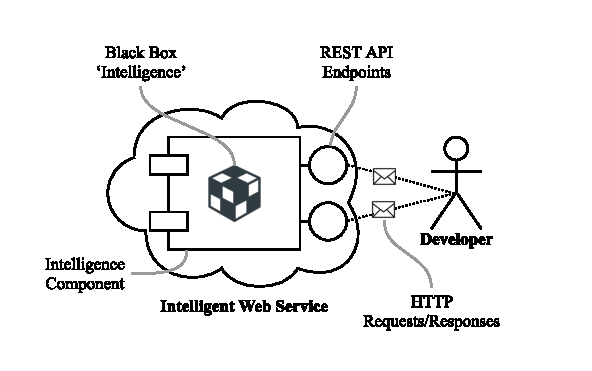
\includegraphics{cloud-intelliegnce-service}
\end{figure}

 
The general workflow of a \gls{cis} is  simple: a developer accesses a \gls{cis} component via \glsac{rest}/\glsac{soap} \gls{api}(s). For their given input, they receive an intelligent-like response typically serialised as \glsac{json}/\glsac{xml}. We note the intelligence component masks its `intelligence' through a black-box: in recent years, there is a rise in providing human-level intelligence via crowdsourcing Internet marketplaces such as Amazon Mechanical Turk~\citep{MTurk:Home} or ScaleAPI~\citep{ScaleAPI:Home}. Thus, a \gls{cis} may be powered by varying degrees of intelligence: human intelligence, machine learning, data mining or even intelligence by brute-force.

While there are different types of \glspl{cis} evident (such as OCR transcription, text-to-speech and speech-to-text, object categorisation, object comparison, natural language processing etc.), we scope the work investigated in this study to \glspl{cvcis}~\citep{GoogleCloud:Home,Azure:Home,AWS:Home,Pixlab:Home,IBM:Home,Cloudsight:Home,Clarifai:Home,DeepAI:Home,Imagaa:Home,Talkwaler:Home,Kairos:Home,Cognitec:Home,Affectiva:Home}. The ubiquity of \glspl{cvcis} is exemplified through evermore growing applications that use these \glspl{api}: aiding the vision-impaired \citep{Reis:2018cp,daMotaSilveira:2017vp}, accounting  \citep{Marshall:2018uj}, data analytics \citep{Iyengar:2017fb}, and student education \citep{Dibia:2017iy}. Moreover, we refer to its growing adoption in developer circles within \cref{fig:introduction:stackoverflow-trends}.